\chapter{Технологический раздел}
\label{cha:impl}
В данном разделе представлены средства разработки программного
обеспечения, детали реализации.

\section{Средства реализации}

Основным средством разработки является язык программирования. Был выбран язык программирования C++. Данный выбор обоснован высокой скоростью работы языка, поддержкой объектно-ориентированного подхода программирования и строгой типизаций \cite{cpplang}. Для написания шейдеров использован язык программирования GLSL, который поддерживается большинством современных видеокарт.

В связи с гибкой архитектурой приложения возможна быстрая интеграция любой библиотеки графического интерфейса (GUI). Было принято решение использовать Free GLUT и ImGui, которые предоставляет базовый набор графических компонентов и функций создания окна,  поддерживают платформы Linux, Windows, macOS и другие \cite{imgui}. 

Для поддержания качества кода было принято использовать инструменты статического анализа кода cpplint\cite{cpplint} и cppcheck\cite{cppcheck}, отладчик использования памяти valgrind\cite{valgrind}. 

\section{Детали реализации алгоритмов}

\subsection{Формирование изображения, буфера глубины и скорости}

Для формирования формирования буферов изображения, глубины и скорости используется шейдер, представленный на листинге \ref{lst:zbuffer.vs}, реализующий модификацию алгоритма удаления невидимых плоскостей с помощью z буфера. Для работа шейдера в него подаются точки полигона, z буфер, буфер скоростей, буфер кадра, ширина и высота буферов, цвет закраски полигона, матрица преобразования в момент времени $t$, обратная матрица преобразований в момент времени $t$, матрица преобразования в момент времени $t - \Delta T$, где $\Delta T$ - время выдержки.
% \begin{figure}[H]    
        \lstinputlisting[
                language=C,
                caption=Шейдер формирования изображения\, буфера глубины и скорости для единичного полигона,
                label=lst:zbuffer.vs,
                ]{code/shaders/zbuffer.cl}
% \end{figure}

% \subsection{Пространственные преобразования}

% В графическом модуле реализованы основные манипуляции со сценой, в том числе и формирование преобразований для каждого объекта и активной камеры. На листинге \ref{lst:cameraTransf} представлено формирование преобразования камеры. Для формирования преобразования анализируется положение и поворот камеры в пространстве сцены в определенный момент времени. 

% \lstinputlisting[language=C,caption=Формирование преобразования камеры,label=lst:cameraTransf]{code/other/cameraTransf.cpp}

% На листинге \ref{lst:cameraTransf} представлено формирование преобразования объекта. Для формирования преобразования анализируется положение, поворот, и масштабирование объекта в пространстве сцены в определенный момент времени. 

% \lstinputlisting[language=C,caption=Формирование преобразования объекта,label=lst:objectTransf]{code/other/objectTransf.cpp}

% \subsection{Буфер скорости пикселей}

% Для формирования буфера скорости пикселей используется конвейер из вершинного и фрагментного шейдеров. Вершинный шейдер вычисляет положение вершины в два момента времени, соответствующие началу и концу выдержки изображения. Данный шейдер представлен на листинге \ref{lst:velocity.vs}.

% \begin{figure}[H]    
%         \lstinputlisting[
%                 language=C,
%                 caption=Вершинный шейдер формирования буфера скорости,
%                 label=lst:velocity.vs,
%                 ]{code/shaders/velocity.vs.glsl}
% \end{figure}


% Полученные положения интерполируются по всему полигону и для каждого пикселя полигона вычисляется разница начального и конечного положения пикселя в пространстве экрана c помощью фрагментного шейдера. Данная разница является скоростью пикселя и заносится в результирующий буфер. Данный шейдер представлен на листинге \ref{lst:velocity.fs}. 



% \lstinputlisting[language=C,caption=Фрагментный шейдер формирования буфера скорости,label=lst:velocity.fs]{code/shaders/velocity.fs.glsl}



\subsection{Формирования смаза с помощью скорости пикселя}

Для формирования смаза с помощью скорости пикселя используются буфер изображения и буфер скорости пикселей, полученные ранее. Для применения фрагментного шейдера для каждого пикселя буфера изображения отрисовывается единичный полигон, занимающий всё пространство экрана. Также в шейдер передается константа $S$ - максимальное количество анализируемых пикселей для формирования смаза. Данный шейдер представлен на листинге \ref{lst:pixelblur.fs}. 

\lstinputlisting[language=C,caption=Фрагментный шейдер формирования смаза с помощью скорости пикселя,label=lst:pixelblur.fs]{code/shaders/pixelBlur.fs.glsl}


\subsection{Формирования смаза помощью максимальной скорости движения участка изображения и буфера глубины}

Формирования буфера максимальной скорости движения участков изображения происходит в два этапа. На первом этапе формируется буфер скорости движения участков изображения. В данный шейдер передается буфер скорости, сформированный ранее и размер участка $k \times k$ в пикселях. Данный шейдер представлен на листинге \ref{lst:tile.fs}. 


\lstinputlisting[language=C,caption=Фрагментный шейдер формирования буфера скорости движения участков изображения,label=lst:tile.fs]{code/shaders/tileMax.fs.glsl}

Следующим этапом формируется  буфер максимальной скорости движения участков изображения с помощью ранее вычисленного буфера  скорости движения участков изображения. Фрагментный шейдер представлен на листинге \ref{lst:neighborMax.fs}.

\lstinputlisting[language=C,caption=Фрагментный шейдер формирования буфера максимальной скорости движения участка изображения,label=lst:neighborMax.fs]{code/shaders/neighborMax.fs.glsl}

Фрагментный шейдер формирования смаза с помощью максимальной скорости движения участка изображения и буфера глубины представлен на листинге \ref{lst:gatherAll.fs}.


\lstinputlisting[language=C,caption=Фрагментный шейдер формирования смаза с помощью максимальной скорости движения участка изображения и буфера глубины,label=lst:gatherAll.fs]{code/shaders/gatherAll.fs.glsl}



\section{Графический интерфейс}

Был разработан графический интерфейс приложения, который представлен на рисунке \ref{fig:gui_window}. 

\begin{figure}[h]
    \centering
    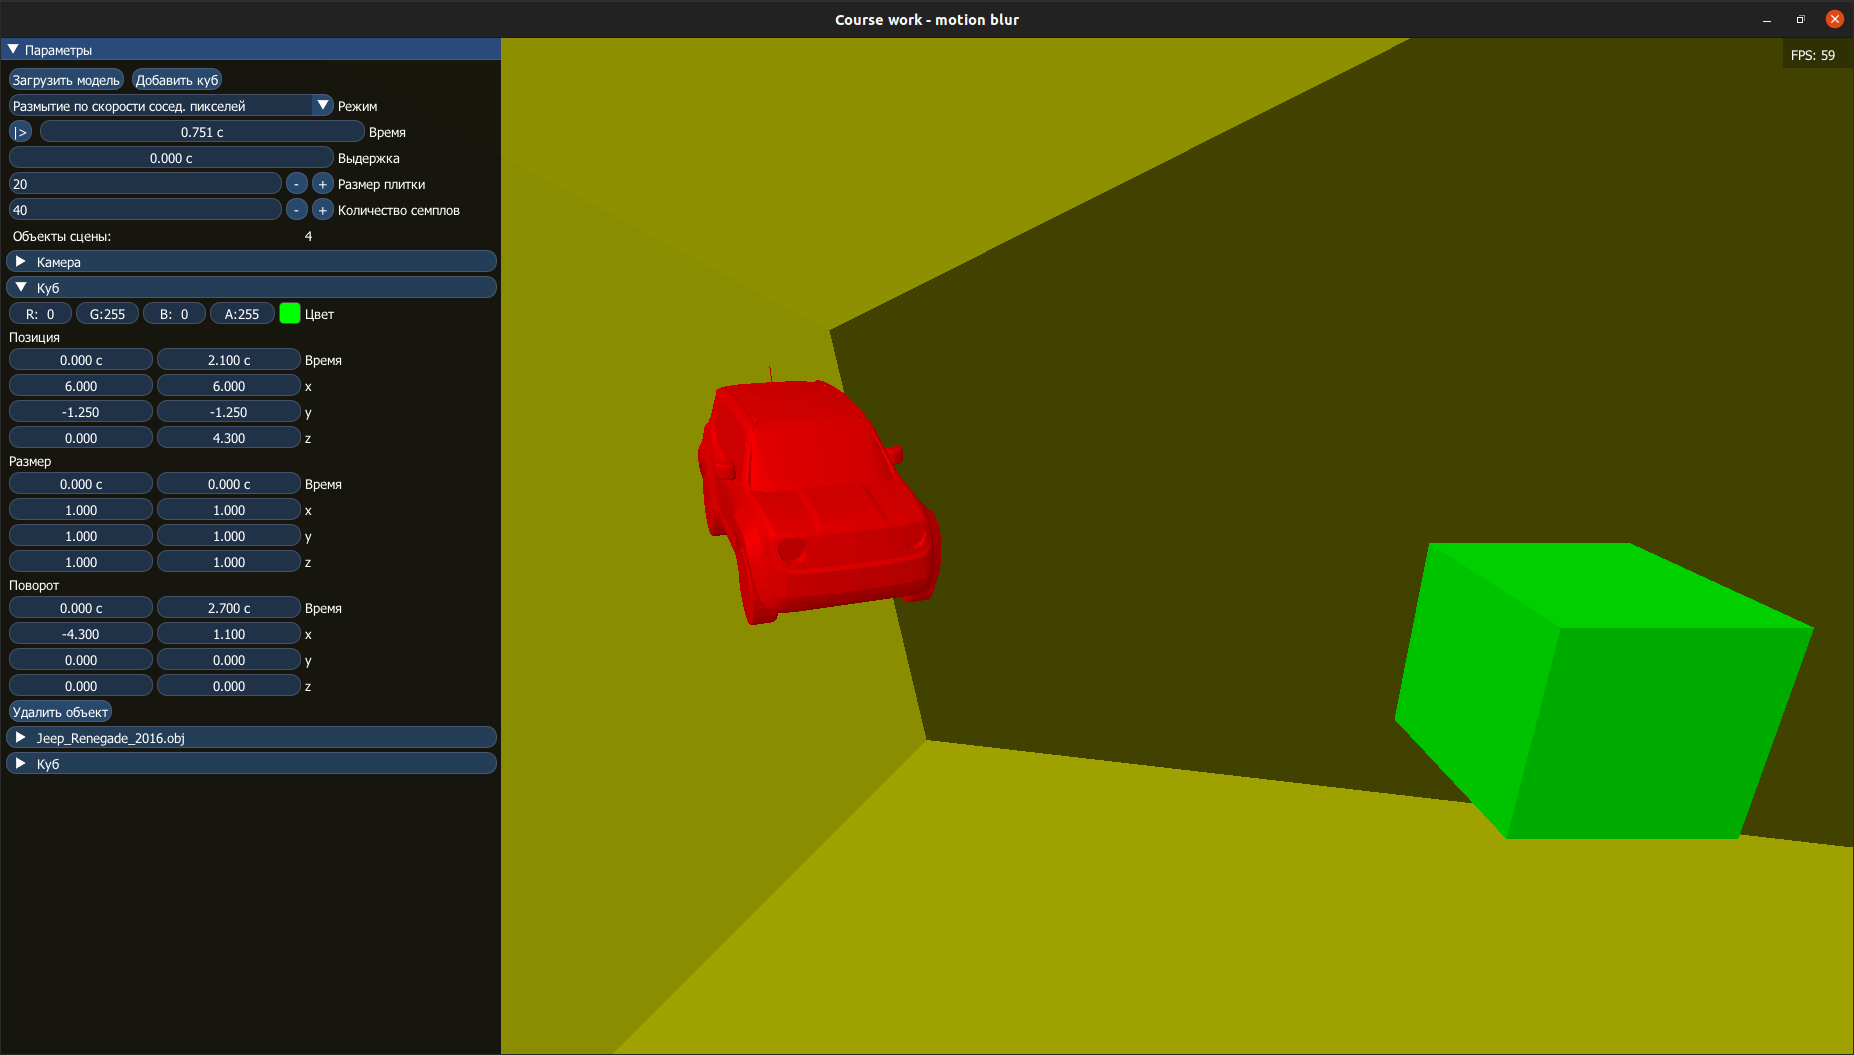
\includegraphics[width=0.9\columnwidth]{img/gui/common_new.png}
    \caption{Общий вид окна}
    \label{fig:gui_window}
\end{figure}


В правой половине окна расположен предпросмотр сцены. В левой половине список объектов сцены и параметры в виде вкладок. На каждой вкладке можно настроить начальное и конечные время анимации и поворот, масштаб, перемещение объекта.
Интерфейс предоставляет возможность просмотреть один из следующих выводов программы:
\begin{itemize}
    \item размытие движения с помощью скорости пикселя;
    \item размытие движения с помощью максимальной скорости
    движения участка изображения и буфера глубины;
    \item буфер кадра -- изображение без размытия;
    \item буфер глубины;
    \item буфер скорости пикселей;
    \item буфер скорости движения участка изображения;
    \item буфер максимальной скорости движения участка изображения.
\end{itemize}

На рисунке \ref{fig:result_buffers} представлены визуализации буферов.



\begin{figure}[h]
    \centering
    \begin{minipage}[h]{0.49\linewidth}
        \center{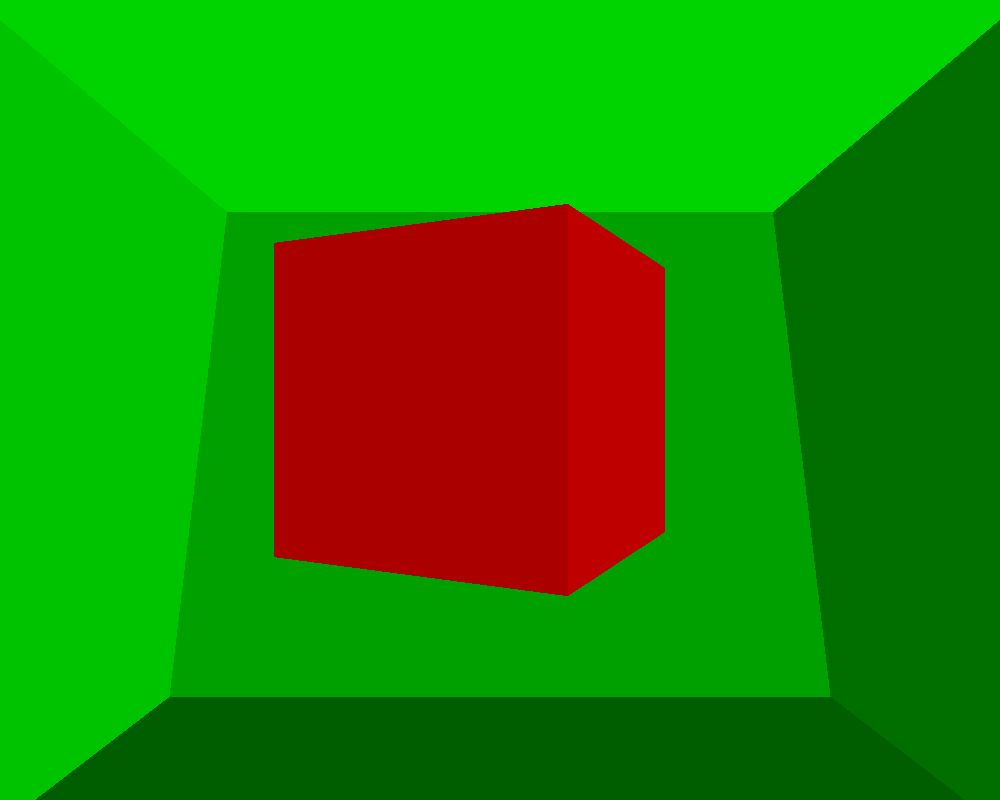
\includegraphics[width=0.8\linewidth]{img/screenshots/t1/color.png} \\ а)}
    \end{minipage}
    \hfill
    \begin{minipage}[h]{0.49\linewidth}
        \center{
\includegraphics[width=0.8\linewidth]{img/screenshots/t1/depth.png} \\ б)}
    \end{minipage}

    \begin{minipage}[h]{0.49\linewidth}
        \center{
\includegraphics[width=0.8\linewidth]{img/screenshots/t1/velocity.png} \\ в)}
    \end{minipage}
    \hfill
    \begin{minipage}[h]{0.49\linewidth}
        \center{
\includegraphics[width=0.8\linewidth]{img/screenshots/t1/neibor.png} \\ г)}
    \end{minipage}


    \begin{minipage}[h]{0.49\linewidth}
        \center{
\includegraphics[width=0.8\linewidth]{img/screenshots/t1/maxneibor.png} \\ д)}
    \end{minipage}
    \hfill
    \begin{minipage}[h]{0.49\linewidth}
        \center{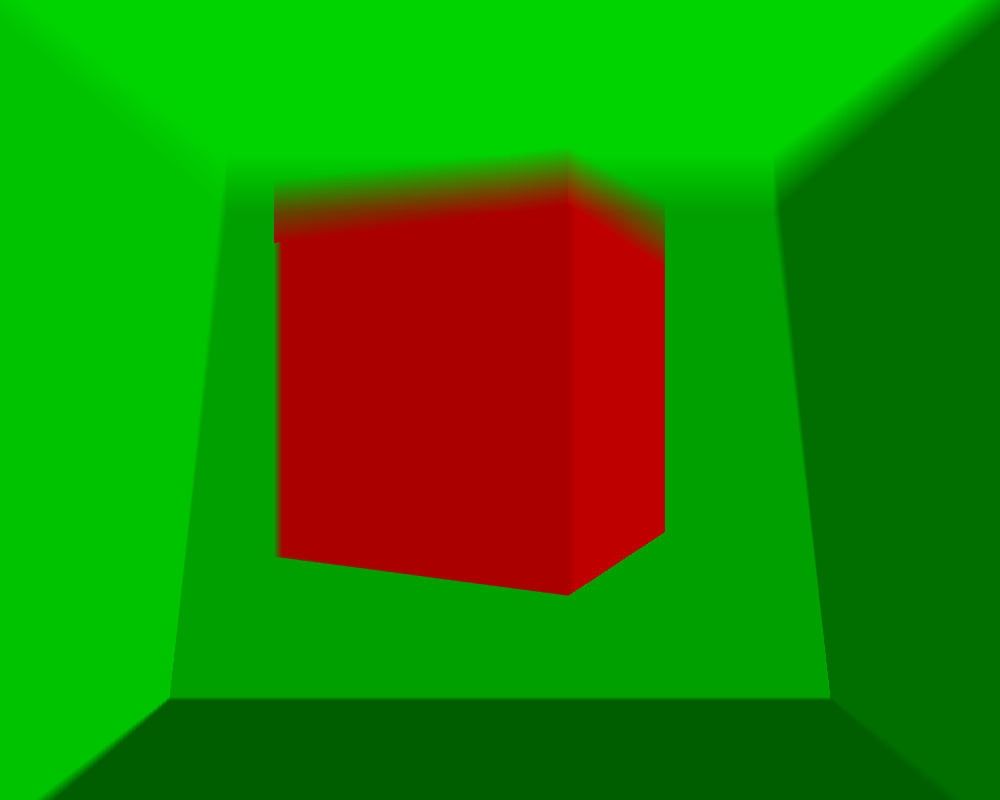
\includegraphics[width=0.8\linewidth]{img/screenshots/t1/pixelblur.png} \\ е)}
    \end{minipage}

    \begin{minipage}[h]{0.49\linewidth}
        \center{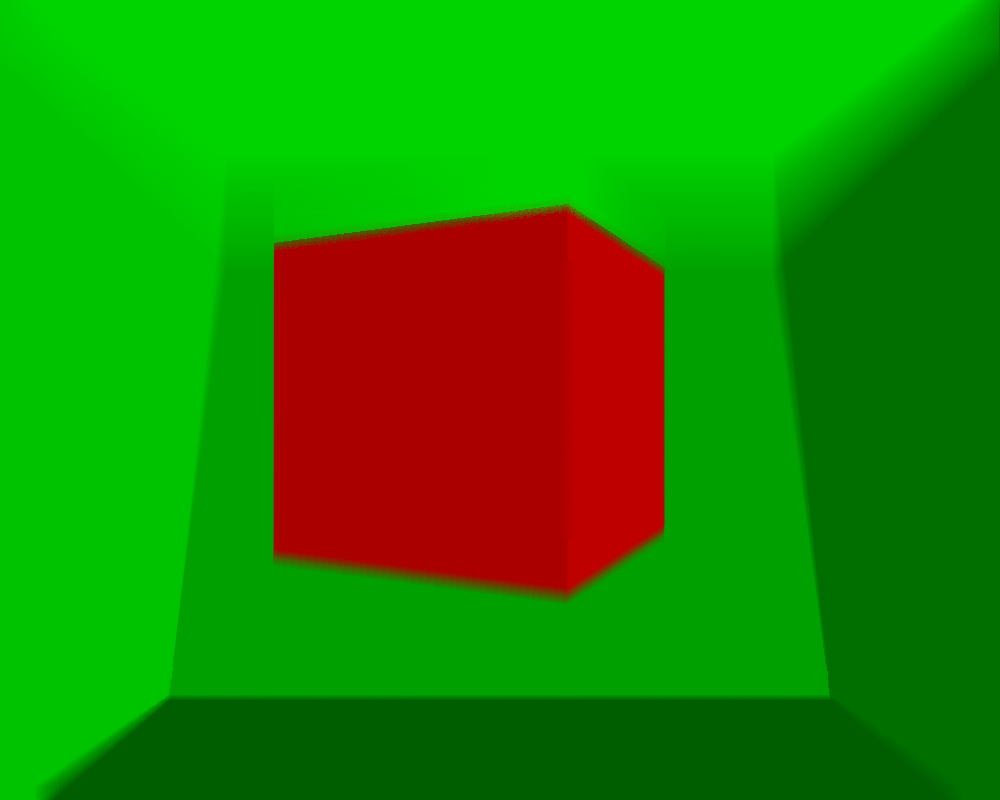
\includegraphics[width=0.8\linewidth]{img/screenshots/t1/mcguire.png} \\ ж)}
    \end{minipage}


    \caption{Результат работы программы. \\ а) Буфер кадра б) Буфер глубины в) Буфер скорости г) Буфер скорости участка \\ д) Буфер максимальной скорости участков  e) Размытие по скорости пикселя \\ ж) Размытие по максимальной скорости участка и буферу скорости  }
    \label{fig:result_buffers}
\end{figure} 


% В данном разделе описано изготовление и требование всячины. Кстати,
% в Latex нужно эскейпить подчёркивание (писать <<\verb|some\_function|>> для \Code{some\_function}).

% \ifPDFTeX
% Для вставки кода есть пакет \Code{listings}. К сожалению, пакет \Code{listings} всё ещё
% работает криво при появлении в листинге русских букв и кодировке исходников utf-8.
% В данном примере он (увы) на лету конвертируется в koi-8 в ходе сборки pdf.

% Есть альтернатива \Code{listingsutf8}, однако она работает лишь с
% \Code{\textbackslash{}lstinputlisting}, но не с окружением \Code{\textbackslash{}lstlisting}

% Вот так можно вставлять псевдокод (питоноподобный язык определен в \Code{listings.inc.tex}):

% \begin{lstlisting}[style=pseudocode,caption={Алгоритм оценки дипломных работ}]
% def EvaluateDiplomas():
%     for each student in Masters:
%         student.Mark := 5
%     for each student in Engineers:
%         if Good(student):
%             student.Mark := 5
%         else:
%             student.Mark := 4
% \end{lstlisting}

% Еще в шаблоне определен псевдоязык для BNF:

% \begin{lstlisting}[style=grammar,basicstyle=\small,caption={Грамматика}]
%   ifstmt -> "if" "(" expression ")" stmt |
%             "if" "(" expression ")" stmt1 "else" stmt2
%   number -> digit digit*
% \end{lstlisting}

% В листинге~\ref{lst:sample01} работают русские буквы. Сильная магия. Однако, работает
% только во включаемых файлах, прямо в \TeX{} нельзя.

% % Обратите внимание, что включается не ../src/..., а inc/src/...
% % В Makefile есть соответствующее правило для inc/src/*,
% % которое копирует исходные файлы из ../src и конвертирует из UTF-8 в KOI8-R.
% % Кстати, поэтому использовать можно только русские буквы и ASCII,
% % весь остальной UTF-8 вроде CJK и египетских иероглифов -- нельзя.

% \lstinputlisting[language=C,caption=Пример (\Code{test.c}),label=lst:sample01]{inc/src/test.c}

% \else

% Для вставки кода есть пакет \texttt{minted}. Он хорош всем кроме: необходимости Python (есть во всех нормальных (нет, Windows, я не про тебя) ОС) и Pygments и того, что нормально работает лишь в \XeLaTeX.

% \ifdefined\NoMinted
% Но к сожалению, у вас, по-видимому, не установлен Python или pygmentize.
% \else
% Можно пользоваться расширенным BFN:

% \begin{listing}[H]
% \begin{ebnfcode}
%  letter = "A" | "B" | "C" | "D" | "E" | "F" | "G"
%        | "H" | "I" | "J" | "K" | "L" | "M" | "N"
%        | "O" | "P" | "Q" | "R" | "S" | "T" | "U"
%        | "V" | "W" | "X" | "Y" | "Z" ;
% digit = "0" | "1" | "2" | "3" | "4" | "5" | "6" | "7" | "8" | "9" ;
% symbol = "[" | "]" | "{" | "}" | "(" | ")" | "<" | ">"
%        | "'" | '"' | "=" | "|" | "." | "," | ";" ;
% character = letter | digit | symbol | "_" ;
 
% identifier = letter , { letter | digit | "_" } ;
% terminal = "'" , character , { character } , "'" 
%          | '"' , character , { character } , '"' ;
 
% lhs = identifier ;
% rhs = identifier
%      | terminal
%      | "[" , rhs , "]"
%      | "{" , rhs , "}"
%      | "(" , rhs , ")"
%      | rhs , "|" , rhs
%      | rhs , "," , rhs ;
 
% rule = lhs , "=" , rhs , ";" ;
% grammar = { rule } ;
% \end{ebnfcode}
% \caption{EBNF определённый через EBNF}
% \label{lst:ebnf}
% \end{listing}

% А вот в листинге \ref{lst:c} на языке C работают русские комменты. Спасибо Pygments и Minted за это.

% \begin{listing}[H]
% \cfile{inc/src/test.c}
% \caption{Пример — test.c} 
% \end{listing}
% \label{lst:c}

% \fi
% \fi
% % Для вставки реального кода лучше использовать \texttt{\textbackslash lstinputlisting} (который понимает
% % UTF8) и стили \Code{realcode} либо \Code{simplecode} (в зависимости от размера куска).




% Можно также использовать окружение \Code{verbatim}, если \Code{listings} чем-то не
% устраивает. Только следует помнить, что табы в нём <<съедаются>>. Существует так же команда \Code{\textbackslash{}verbatiminput} для вставки файла.

% \begin{verbatim}
% a_b = a + b; // русский комментарий
% if (a_b > 0)
%     a_b = 0;
% \end{verbatim}

%%% Local Variables:
%%% mode: latex
%%% TeX-master: "rpz"
%%% End:
